\documentclass[english,,man]{apa6}
\usepackage{lmodern}
\usepackage{amssymb,amsmath}
\usepackage{ifxetex,ifluatex}
\usepackage{fixltx2e} % provides \textsubscript
\ifnum 0\ifxetex 1\fi\ifluatex 1\fi=0 % if pdftex
  \usepackage[T1]{fontenc}
  \usepackage[utf8]{inputenc}
\else % if luatex or xelatex
  \ifxetex
    \usepackage{mathspec}
  \else
    \usepackage{fontspec}
  \fi
  \defaultfontfeatures{Ligatures=TeX,Scale=MatchLowercase}
\fi
% use upquote if available, for straight quotes in verbatim environments
\IfFileExists{upquote.sty}{\usepackage{upquote}}{}
% use microtype if available
\IfFileExists{microtype.sty}{%
\usepackage{microtype}
\UseMicrotypeSet[protrusion]{basicmath} % disable protrusion for tt fonts
}{}
\usepackage{hyperref}
\hypersetup{unicode=true,
            pdftitle={A Simple, Dynamic Extension of Temporal Motivation Theory},
            pdfauthor={Christopher R. Dishop},
            pdfborder={0 0 0},
            breaklinks=true}
\urlstyle{same}  % don't use monospace font for urls
\ifnum 0\ifxetex 1\fi\ifluatex 1\fi=0 % if pdftex
  \usepackage[shorthands=off,main=english]{babel}
\else
  \usepackage{polyglossia}
  \setmainlanguage[]{english}
\fi
\usepackage{graphicx,grffile}
\makeatletter
\def\maxwidth{\ifdim\Gin@nat@width>\linewidth\linewidth\else\Gin@nat@width\fi}
\def\maxheight{\ifdim\Gin@nat@height>\textheight\textheight\else\Gin@nat@height\fi}
\makeatother
% Scale images if necessary, so that they will not overflow the page
% margins by default, and it is still possible to overwrite the defaults
% using explicit options in \includegraphics[width, height, ...]{}
\setkeys{Gin}{width=\maxwidth,height=\maxheight,keepaspectratio}
\IfFileExists{parskip.sty}{%
\usepackage{parskip}
}{% else
\setlength{\parindent}{0pt}
\setlength{\parskip}{6pt plus 2pt minus 1pt}
}
\setlength{\emergencystretch}{3em}  % prevent overfull lines
\providecommand{\tightlist}{%
  \setlength{\itemsep}{0pt}\setlength{\parskip}{0pt}}
\setcounter{secnumdepth}{0}
% Redefines (sub)paragraphs to behave more like sections
\ifx\paragraph\undefined\else
\let\oldparagraph\paragraph
\renewcommand{\paragraph}[1]{\oldparagraph{#1}\mbox{}}
\fi
\ifx\subparagraph\undefined\else
\let\oldsubparagraph\subparagraph
\renewcommand{\subparagraph}[1]{\oldsubparagraph{#1}\mbox{}}
\fi

%%% Use protect on footnotes to avoid problems with footnotes in titles
\let\rmarkdownfootnote\footnote%
\def\footnote{\protect\rmarkdownfootnote}


  \title{A Simple, Dynamic Extension of Temporal Motivation Theory}
    \author{Christopher R. Dishop\textsuperscript{1}}
    \date{}
  
\shorttitle{GOAL SAMPLING}
\affiliation{
\vspace{0.5cm}
\textsuperscript{1} Michigan State University}
\usepackage{csquotes}
\usepackage{upgreek}
\captionsetup{font=singlespacing,justification=justified}

\usepackage{longtable}
\usepackage{lscape}
\usepackage{multirow}
\usepackage{tabularx}
\usepackage[flushleft]{threeparttable}
\usepackage{threeparttablex}

\newenvironment{lltable}{\begin{landscape}\begin{center}\begin{ThreePartTable}}{\end{ThreePartTable}\end{center}\end{landscape}}

\makeatletter
\newcommand\LastLTentrywidth{1em}
\newlength\longtablewidth
\setlength{\longtablewidth}{1in}
\newcommand{\getlongtablewidth}{\begingroup \ifcsname LT@\roman{LT@tables}\endcsname \global\longtablewidth=0pt \renewcommand{\LT@entry}[2]{\global\advance\longtablewidth by ##2\relax\gdef\LastLTentrywidth{##2}}\@nameuse{LT@\roman{LT@tables}} \fi \endgroup}


\DeclareDelayedFloatFlavor{ThreePartTable}{table}
\DeclareDelayedFloatFlavor{lltable}{table}
\DeclareDelayedFloatFlavor*{longtable}{table}
\makeatletter
\renewcommand{\efloat@iwrite}[1]{\immediate\expandafter\protected@write\csname efloat@post#1\endcsname{}}
\makeatother
\usepackage{lineno}

\linenumbers

\authornote{Christopher R. Dishop, Department of Psychology,
Michigan State University

Correspondence concerning this article should be addressed to
Christopher R. Dishop, 316 Physics Rd \#348, East Lansing, MI 48824.
E-mail:
\href{mailto:dishopch@msu.edu}{\nolinkurl{dishopch@msu.edu}}}

\abstract{
Steel and Konig's (2006) temporal motivation theory (TMT) has been
criticized for its static representation and neglect of the environment.
In this paper, I develop goal sampling theory (GST) to appease these
criticisms and extend our understanding of goal choices beyond momentary
preferences and into dynamic updating and global sampling behavior
across time. GST draws from temporal motivational theory (TMT), sampling
models of impression formation, and organizational theory on how the
environment constrains behavior and situates aspects of each into a
formal representation of goal sampling. Doing so addresses the
limitations of our prior thinking, introduces new concepts and
predictions, and provides a mathematical framework that lends itself to
computational modeling.


}

\usepackage{amsthm}
\newtheorem{theorem}{Theorem}[section]
\newtheorem{lemma}{Lemma}[section]
\theoremstyle{definition}
\newtheorem{definition}{Definition}[section]
\newtheorem{corollary}{Corollary}[section]
\newtheorem{proposition}{Proposition}[section]
\theoremstyle{definition}
\newtheorem{example}{Example}[section]
\theoremstyle{definition}
\newtheorem{exercise}{Exercise}[section]
\theoremstyle{remark}
\newtheorem*{remark}{Remark}
\newtheorem*{solution}{Solution}
\begin{document}
\maketitle

Employees often face multiple, conflicting goals as they complete their
work day. Core tasks, such as skill acquisition and networking
opportunities, projects, and reports flood employee experiences while
superficial demands, such as emails, meetings, and phone calls threaten
to emerge at any moment. In these environments, how do individuals
decide which goal to pursue? What process guides their goal sampling
behavior over time? Goal choice theories often evoke utility functions
(Keeney \& Raiffa, 1976; Steel \& König, 2006; Von Winterfeldt \&
Edwards, 1982) to explain this operation, such that employees choose
goal \enquote{A} over goal \enquote{B} to the extent that \enquote{A}
produces greater utility. These explanations are among the most
actionable organizational theories due to their concrete predictions
(Miner, 1980; Van Eerde \& Thierry, 1996a), but they have largely
focused on single, static equations that neglect how the decision
process updates and evolves alongide the constraints of the environment
(Busemeyer, Townsend, \& Stout, 2002; Luce, 1995). Goal choice theories
across psychology, economics, and sociology largely agree on the
necessary function parameters (Steel \& König, 2006), therefore it is
time to move beyond specifying a single equation and build a theory that
describes the \emph{dynamics} of goal choice updating.

I present a theory of goal choice that subsumes prior work and embeds
the individual utility function in a framework that makes both competing
and complimentary predictions. The framework is grounded in experience
sampling (Denrell, 2005, 2007) where the likelihood of choosing a goal
is based not only on a utility function, but also on experiences, the
constraints of where utility was in the past, and the environment.
Specifically, individuals choose only among goals made available by the
environment and this choice depends on whether prior experiences with
each were positive or negative. Although utility functions (referred to
hereafter as \(U\) functions) influence this process, the theory
presented here shows how they are only one piece to a larger goal
decision framework. Newell (1973) and Meehl (1967, 1978) argued that, if
theories are to be useful, they require integrating individual
components and specifying a \enquote{control structure,} which is a
computer programming phrase used to describe the flow across an entire
block of code rather than specific functions or variable assignments.

In this paper I unpack goal sampling theory (GST), a theory that extends
prior work and uses a simple sampling model to unify different
perspectives and explain goal choice updating. Its purpose is to extend
work by Steel and König (2006) by incorporating dynamics. Prior work
includes time as a parameter in the various utility equations, but
simply including time in the parameter space does not make the equation
dynamic. Dynamics, stated simply, refers to a branch of
mathematics/mechanics where the crucial notion is memory -- the past
constrains what happens next (Kondrashov, 2016). Once dynamics is
represented in the equations, additional concepts emerge that address
assumptions and limitations present in our prior thinking related to
goal choices -- those will be discussed within each individual section
below.

The following paper moves sequentially, rather than presenting the
entire theoretical framework upfront, to simplify the equations and
clearly specify what each aspect represents. Please note that the paper
was written to (hopefully) facilitate clarity: GST is discussed in full
only after presenting a variety of much simpler equations surrounding
prior goal choice theories, their limitations, and components that I
hope to improve upon.

\hypertarget{choosing-a-goal}{%
\section{Choosing a Goal}\label{choosing-a-goal}}

Goals refer to internal representations of desired states (Austin \&
Vancouver, 1996), and the organizational goal-decision literature is
concerned with how employees choose which goal to pursue. This notion is
distinct from goal-striving, which describes effort and performance
strategies usually in the pursuit of a single goal (for exceptions, see
Schmidt \& DeShon, 2007; Vancouver, Weinhardt, \& Schmidt, 2010).
Theories of goal choice and decision making are present in economics,
psychology, and sociology, and are nicely integrated by Steel and König
(2006). Their temporal motivation theory (TMT) incorporates hyperbolic
discounting, expectancy theory, cumulative prospect theory, and need
theory into an integrated \(U\) function that predicts goal choice. The
details of those theories are not crucial here, as each delivers a
variant of a utility equation, such that:

\begin{equation}
U = f(X_{theory})
\end{equation} \noindent where \(U\) represents utility, or a preference
for a certain goal, and \(X\) is a set of variables whose formal
representation depends on the theory. The set of variables across each
theory, \(X\), are not the focus of this paper so they will only be
briefly described here. Core variables in the set typically include
expectancy, valence, and deadline/outcome time. Expectancy refers to a
subjective belief about the likelihood of achieving a goal. Valence is
how much an individual values the outcome that follows goal attainment,
and time in TMT refers to when the outcome is received (how distant the
reward is). As stated in Steel and König (2006), the consistency of
\(U\) functions across fields for predicting goal choices is greater
than one would assume, and I therefore use \(U\) as a starting point to
expand on. A common critique of these functions, however, is their
neglect of the environment (Johns, 2018; Kanfer \& Chen, 2016; Kerr,
1975; Simon, 1956). The next section presents the first extension of
\(U\) by incorporating the environment.

\hypertarget{the-environment}{%
\section{The Environment}\label{the-environment}}

Any description of behavior must account for the environment in which it
occurs (Simon, 1992) because the environment constrains what actions are
possible (Cappelli, 1991; Greeno, 1994; Simon, 1956). Although prominent
authors have repeatedly critiqued the limited attention to context in
organizational research (Johns, 2006; Kanfer \& Chen, 2016), there are
many examples that highlight its relevance in other disciplines.

Studies of animal behavior have repeatedly shown that the environment
influences basic physiology. Signs of healthy brain development, such as
improved plasticity and neurotrophic functioning, are greater in mice
raised in enriched environments (e.g., cages with toys and other mice)
compared to those raised in isolation (Duman, 2009). Beyond basic
physiological functioning, context also plays a role in decision-making.
Douglas, Bateson, Walsh, Bédué, and Edwards (2012) trained pigs to
approach a hatch following a certain sound but avoid the hatch after a
different, second sound. The authors were then interested in what would
happen when they introduced a novel tone. Pigs raised in barren
environments showed no differences in their approach/avoidance behavior,
whereas pigs that were raised in comfortable, social, and playful
environments were more likely to demonstrate approach behavior following
the novel tone. This effect has also been replicated across a variety of
other animals (Brydges, Leach, Nicol, Wright, \& Bateson, 2011;
Matheson, Asher, \& Bateson, 2008; Salmeto et al., 2011).

A key insight that will be discussed throughout this paper is that the
environment acts like a leash, making certain behaviors more or less
likely (but not guaranteed). For example, Worthy, Maddox, and Markman
(2007) asked college students to sequentially choose a single card from
one of two decks. The authors manipulated whether the focus of the task
was to gain points or avoid loosing points based on the values of the
drawn cards. Moreover, they also manipulated the framing of the payout
structure by telling participants that they would either be entered into
a lottery if they achieved a certain amount of points (promotion) or
removed from the lottery if they failed to sustain those points
(prevention). One of the decks returned greater values initially but was
ultimately worse to choose from, whereas the other was more valuable to
choose from in the long run but provided bad cards initially. The
authors were thus interested in the card deck sampling behavior of the
participants. Participants explored more (sampled more from the
\enquote{initially bad} deck) under regulatory match manipulations, or
when gain was paired with promotion and loss was paired with prevention.
Exploitive behavior (sampling from the \enquote{initially good} deck),
conversely, emerged among participants under regulatory mismatch
conditions, or when gain was paired with prevention and loss was paired
with promotion.

These results demonstrate that the environment enhances or diminishes
the probability of certain behavior patterns. The probability of
choosing from the deck \enquote{initially bad} is constrained by both
the reward it provides and the nature of the situation.
Exploratory/exploitive behaviors thus become more or less likely
depending on context. Note that I am referring to the
promotion/prevention and gain/loss framing as the \enquote{environment}
because, despite there being literature on a regulatory focus individual
difference (Crowe \& Higgins, 1997), they were used as part of the task
and therefore align more with the literature on job characteristics than
individuals differences (Hackman \& Oldham, 1976).

The aforementioned animal behavior studies could be construed as
evidence that \enquote{positive} environments produce \enquote{positive}
outcomes, but Worthy et al. (2007) also show that what we need to
consider with respect to the environment is what it
constrains/facilitates, not whether it is positive or negative. There
are numerous examples where seemingly positive environments actually
produce worse outcomes. Job autonomy, for instance, sometimes leads to
lower creativity, and job richness can lead to stress in some cases
(Johns, 2010). What matters is that the environment increases or reduces
the probability of certain behavior patterns regardless of whether or
not they are positive. For example, overconfidence, while negative in
some domains, is adaptable in environments that are novel,
unpredictable, or poorly understood (Johnson \& Fowler, 2011).

Contrary to the environment's limited appearance in organizational field
work, we find it highlighted in many psychological theories. Events
systems theory predicts that many organizational changes arise from
critical events that are novel or disruptive (Morgeson, Mitchell, \&
Liu, 2015), which then explain relationships between seemingly
unconnected levels of an organization. Tett and Burnett's (2003) trait
activation theory specifies features of the environment that constrain
or facilitate job performance. For example, a \enquote{job demand to
interact with others might elevate the performance of an extrovert,
whereas the presence of random others or physical isolation might
respectively distract or constrain this person in terms of performance}
(Johns 2018 p.~25). Gigerenzer and the ABC group study ecological
rationality, or fast decision-making with respect to constraints imposed
by the environment (Gigerenzer, Todd, \& ABC Research Group, 1999).
Finally, Grandey's model of emotional labor acknowledges that job
environments, including interactions with customers and the behavioral
expectations of the organization, change the probability of emotional
responses in employees (Grandey, 2000; Grandey \& Gabriel, 2015). A
common feature of theories that include the environment, therefore, is
acknowledging the constraints it places on behavior.

I argue that the environment is important for goal choices as well.
Consider a few examples: An employee has a high utility for goal
\enquote{A} but is forced to work on goal \enquote{B} by their manager;
A co-worker is sick and asks another individual to cover their tasks for
the day; Low performance at a neighboring branch requires an individual
to put off their current work and help train their fellow employees; A
Wi-Fi outage constrains an individual's set of goal options; An email
with a provocative subject line draws an individual's attention away
from their current goal. These examples are simple but are by no means
uncommon, yet they are difficult to represent with only utility.
Moreover, they reveal that some environmental constraints are consistent
but others are random or difficult to predict. Instantiating this notion
into a representation of goal choice, therefore, can be done with
likelihoods, where an individual has a probability of choosing a goal at
a given moment with respect to the environmental constraints. Stated
formally:

\begin{equation}
\Theta_{A} = E * U_{A}
\end{equation} \noindent where \(\Theta_{A}\) represents the likelihood
of choosing goal \enquote{A,} which is a function of both the
environment, \(E\), and the utility of \enquote{A}, \(U_{A}\). If the
environment places restraints on goal \enquote{A} such that it cannot be
sampled, then \(E\) would be zero and the likelihood of choosing
\enquote{A} would also become zero. Although this is a simple
representation of the environment, Meehl (1967) suggested creating
simple formulas such as the one presented despite an incomplete
understanding of the \enquote{true} function (see also Morgan \&
Winship, 2015). We may never be able to adequately capture the
environment, but it is important to represent nonetheless.

\textbf{Strengths of Incorporating the Environment} By specifying
equation two I reveal several strengths of GST that are missing in prior
work. First, prior utility models cannot account for situations like
those presented above where context forces an individual to change
goals. These models either assume that the environment does not matter
or is somehow incorporated into the variables that make up utility
(valence, expectancy, deadline time). This second assumption does work
occasionally -- if, for example, a government shutdown creates new
deadline times -- but it is not amenable to the spectrum of situations
described above.

Second, creating a likelihood function by combining the environment with
utility demonstrates GST's focus on probabilistic goal sampling rather
than a deterministic choice. Researchers use probabilistic terms to
describe valence and expectancy (Van Eerde \& Thierry, 1996b), but prior
formulae for choosing goals imply that two choices at different points
in time should be identical if the values in the set of \(X\) at each
are the same. GST, conversely, acknowledges that goal choices may differ
from one moment compared to another despite equal utility at both. The
environment term, therefore, acts like a mathematical error term and
captures the notion of different goal choices despite identical utility
across time. Probabilitic models are also increasingly popular because
even deterministic systems can create unpredictable behavior (Mitchell,
2009), GST therefore presents a model consistent with the broader
scientific literature.

\textbf{Proposition 1} \emph{Goal sampling at two time points may be
different -- even when utility is exactly the same -- because the
environment forces sampling.}

Finally, emphasizing probability sampling hints that the process must be
studied over time. Although researchers three decades ago were excited
about the increasing prevalence of process explanations in our theories
and longitudinal designs in our investigations (Monge, 1990), authors
today still express disappointment by the static descriptions lingering
in our theories and empirical articles -- even among longitudinal
designs (Cortina, 2016; Cortina, Aguinis, \& DeShon, 2017; DeShon, 2012;
Pitariu \& Ployhart, 2010; Ployhart \& Vandenberg, 2010; Vancouver,
Wang, \& Li, 2018). GST reorients our thinking from a single event to
multiple episodes simply because likelihoods bring to mind a phrase that
implies repetition: \enquote{sampling from a distribution.} That said,
we are still left with a static theory because equation two has no way
of updating over time. In the next section, therefore, I unpack my next
extension: dynamic updating.

\hypertarget{dynamic-updating}{%
\section{Dynamic Updating}\label{dynamic-updating}}

Utility functions have been labeled as time insensitive, static, and
unable to capture dynamic effects (Baumeister, Vohs, \& Oettingen, 2016;
Luce, 1999). Steel and König (2006) respond to calls for a dynamic
representation in TMT by formally including time as a variable in their
\(U\) function, such that positive outcomes far removed produce lower
utility. Incorporating deadlines is appropriate, but simply including
time as a variable does not make the equation dynamic. That is, when the
\(U\) function incorporates deadline time it is still expressed as:

\begin{equation}
U = f(X_{theory})
\end{equation} \noindent but a variable, \(T\), which is the amount of
time until a goal's deadline, is incorporated into the set of \(X\).
Doing so captures subjective time, but it does not represent the process
over time. To do so, we can change the equation to acknowledge two
assumptions: 1) that \(U\) can change over time

\begin{equation}
U_{t}
\end{equation} \noindent and 2) that \(U\) is a function of current
variables in the set of \(X\):

\begin{equation}
f(X_{theory})_{t}
\end{equation} \noindent which gives us the following when we combine
those ideas:

\begin{equation}
U_{t} = f(X_{theory})_{t}.
\end{equation} \noindent That is, utility at time four depends on the
set of variables in \(X\) at time four, but utility at time five can be
different from utility at time four.

We now have a description of utility over time, but this representation
is still not consistent with what researchers would consider dynamic
modeling (Busemeyer, 2018; Voelkle \& Oud, 2015). Utility, as presented
above, is memoryless, where any effects at time \(t\) disappear and are
replaced by new effects at time \(t+1\). Dynamic representations account
for the past, and there are many empirical examples where prior states
carry over into the future. For example, personality shows stability
over time, with test-retest correlations as high as 0.8 (Denissen, Aken,
\& Roberts, 2011). Children retain their delay of gratification
abilities across their lifetime (Tobin \& Graziano, 2010). Goal
discrepancy states show consistency over time (DeShon \& Rench, 2009)
reflecting satiated behavior (Simon, 1956). Team cohesion and
performance have stability coefficients of 0.50 (Mathieu, Kukenberger,
D'innocenzo, \& Reilly, 2015). Finally, Shan (2005) argued that
suspected predictors of economic growth contribute little to the
understanding of an economic trajectory over its own prior behavior.
Indeed, it is difficult to find examples where prior states are not
important to the development of a variable over time. We represent
states with memory mathematically by using autoregressive terms. The
following:

\begin{equation}
U_{(t+1)} = b_0 U_{t}
\end{equation} \noindent expresses utility dynamically, where
\(U_{(t+1)}\) is utility at the next time point and \(b_0\) represents
the coefficient relating current to future utility, which formally
models self-similarity (DeShon, 2012; Vancouver \& Weinhardt, 2012).

\textbf{Strengths of Incorporating Dynamics} Adding this dynamic element
reveals additional strengths of GST. First, utility now has similarity
across time. Prior explanations and models that do not present utility
in this way assume that goal choices are independent at each moment and
any effects at time \(t\) disappear and are replaced by new ones at time
\(t+1\). Although you can describe processes over time in this way,
these explanations amount to no more than compiled snapshots of behavior
that miss the continual flow governing the system (Ilgen \& Hulin,
2000). As stated above, it is difficult to find an occasion where the
prior behavior of a variable is not important to its own development,
and incorporating autoregression presents a more realistic model of
utility.

Models that do not account for the past also imply that utility is
unconstrained across time. That is, utility at time \(t\) can jump to
high or low values at time \(t+1\) irrespective of its position at
\(t\). Although I have not seen a discussion about whether such behavior
is possible for utility, it would be inconsistent with how researchers
in empirical articles describe the variables in the set of \(X\) (Dreher
\& Bretz, 1991; Erez \& Isen, 2002).

\textbf{Proposition 2} \emph{Utility has self similarity across time,
such that a goal's utility at time \(t\) is positively related to its
value at \(t + 1\).}

Of course, understanding a process also requires that we account for
\emph{other} prior states (variables). Prior fluctuations in burnout
predict turnover cognitions (Taylor, Bedeian, Cole, \& Zhang, 2014),
perceived changes in HR systems influence future customer satisfaction
(Piening, Baluch, \& Salge, 2013), and training developments influence
later performance (Kraiger, Ford, \& Salas, 1993). What prior variable
states are important to consider for goal choices? Some indirect
evidence suggests that experiences with goals and their outcomes inform
future decisions. Gambling payoffs influence future bets (Thaler \&
Johnson, 1990). Customers make different choices about consumer items if
their immediately prior experiences are positive rather than negative
(Novemsky \& Dhar, 2005). Task choices are informed by levels of prior
task achievement (Bandura, 2001; Lewin, Dembo, Festinger, \& Sears,
1944). Ackerman's theory of intellectual development connects prior task
success or failure to interests, which then drive future task sampling
(Ackerman, 1996; Reeve, Scherbaum, \& Goldstein, 2015). Finally, social
impressions influence future interactions, such that pleasurable
experiences increase the likelihood of the social group meeting again
(Thibaut \& Kelley, 1959).

To cover these situations we need a way to incorporate experiences
(defined below). In the next section I discuss a sampling model that
helps us do so.

\hypertarget{experience-sampling}{%
\section{Experience Sampling}\label{experience-sampling}}

GST claims that goal experiences, or subjective evaluations of the
feedback and rewards received from sampling a goal, combine with utility
and the environment to drive future goal sampling. The mechanism by
which this happens is drawn from Denrell's (2005; 2007) sampling model
of impression formation, where people are more likely to sample (i.e.,
engage with) others for whom they have positive impressions, but stop
sampling anyone for whom they have negative impressions. GST extends
this notion to goals and experiences with their outcomes. If an
individual receives a subjectively favorable experience from a goal then
its utility increases and the individual becomes more likely to sample
it again in the future. When goals produce unfavorable outcomes,
conversely, individuals stop sampling (with a certain probability).
Relating goal sampling to prior experiences not only facilitates a
dynamic understanding of the process, but it also captures the classic
effects of feedback and reward (Dickinson, 1989; Kerr, 1975; Ludvig,
Bellemare, \& Pearson, 2011; Pinsker, Kupfermann, Castellucci, \&
Kandel, 1970; Rescorla \& Wagner, 1972).

A formal representation of utility updating based on its own prior state
and the sampling experience is as follows:

\begin{equation}
U_{(t+1)} = b_0 U_{t} + b_1 Ep_t
\end{equation} \noindent where \(Ep_t\) represents the experience of a
goal at time \(t\), \(b1\) is the weight relating experience to utility,
and all other terms are defined above.

Utility then influences the probability of sampling alongside the
constraints of the environment at the next time point (\(E_{t+1}\)):

\begin{equation}
\Theta_{(t+1)} = E_{t+1} * {\frac {1}{1 + e^{U_{(t+1)}}}}
\end{equation} \noindent where \(\Theta_{(t+1)}\) represents the
likelihood of sampling at \(t+1\) and all other terms are defined above.
I will thoroughly discuss the components of these equations in later
sections. What is important here is to recognize that we mathematically
represented the following: utility and the goal sampling experience
influence utility at the next time point (equation 8), and at this time
utility combines with the environment to inform the likelihood of goal
sampling (equation 9).

\textbf{Strengths of Incorporating Experience Sampling} Incorporating
experience sampling provides two strengths beyond prior work. First, I
account for the known influence of feedback and reward. Second, GST
captures goal sampling irrespective of goal completion. There are many
examples where individuals can still sample goals even after completing
them, but past utility theories overlook these situations by focusing
only on behavior leading up to goal completion. These implications,
however, can be difficult to see from the equations; I therefore discuss
them with examples below.

GST predicts that goal experiences influence future goal sampling.
Again, an experience in GST is an individual's subjective evaluation of
the feedback or reward a specific goal sample produces. For example,
imagine a professor setting the goal to read 50 pages of a book. After
one sample of this goal she receives feedback in (potentially) many
forms, such as pay, social acknowledgment from others, or feelings
regarding reading itself (e.g., pleasure or exhaustion). GST summarizes
her subjective evaluation of this feedback with a single value: the
experience. If taking action toward the \enquote{read 50 pages} goal
results in a positive experience then the professor is more likely to
sample it again in the future. But if doing so produces a negative
experience then she has a much lower sampling probability. In GST,
therefore, the decision to sample is directly tied to utility and the
accumulated prior experiences on which it is based.

\textbf{Proposition 3} \emph{Goal choices at time \(t\) are positively
related to subjective evaluations of a goal experience at the
immediately prior time point \(t - 1\), such that individuals are more
likely to sample goals that provide a subjectively favorable experience
at \(t - 1\) but less likely to sample goals that provide a subjectively
unfavorable experience at \(t - 1\).}

Second, GST focuses on global sampling behavior and the mechanism just
described applies irrespective of whether or not individuals complete
the goal. Rather, goal completion in GST is viewed as another experience
of sampling. To continue the example, imagine two situations: one where
the professor does \emph{not} complete her goal of reading 50 pages, and
a second where she does complete it. Both of these situations are
samples of the \enquote{50 pages} goal where future sampling depends on
her perceptions of the experience feedback at each sample.

Consider first the situation where she does \emph{not} complete the
goal. If she views this sample as negative because she underperforms,
then sampling the \enquote{50 pages} goal is unlikely moving forward.
But if other positive aspects of reading overwhelm the negative
underperformance, such as the riveting nature of the material or the
tranquility surrounding quiet reading time, then the probability of
future sampling is higher.

Turn now to the situation where she does complete the \enquote{50 pages}
goal. If she views this experience as negative (due to say, exhaustion),
then future sampling is lower than if she finds the experience positive
(due to completing the goal). GST, therefore, focuses on utility
updating and sampling behavior across time due to various experiences
regardless of where the individual lies on their \enquote{goal
completion} continuum. If an individual terminates a goal by completing
it, then it can no longer be sampled in the future. But there are many
cases, the \enquote{read 50 pages} being one, where goal completion does
not remove the goal; GST captures both of these situations.

\textbf{Proposition 4} \emph{The mechanism of goal sampling as presented
in GST is the same irrespective of whether or not the individual has
completed the goal.}

\hypertarget{goal-sampling-theory}{%
\section{Goal Sampling Theory}\label{goal-sampling-theory}}

I have introduced important components for theories of goal choice.
Utility perceptions inform goal preferences in the moment, the
environment constrains which goals are available, and prior experiences
update goal sampling likelihoods. I discussed each individually to avoid
overwhelming the reader with equations, but I now move to the full goal
sampling theory and place these aspects into a \enquote{control
structure} framework to demonstrate how this process develops over time
(Meehl, 1967; Newell, 1973).

In GST, goal choices are viewed as opportunities to sample goals.
Sampling results in an experience, which can be thought of as an
individual's subjective evaluation concerning the feedback or reward it
produces for that specific sample. This experience updates utility,
which then informs the likelihood of sampling that goal again in the
future -- alongside the constraints of the environment. Repeated
sampling is likely when prior experiences are positive and unlikely when
prior experiences are negative (Denrell, 2005), such that individuals
have a low probability of sampling goals that produced poor outcomes in
the past.

The core elements of the theory, therefore, include experiences,
utility, and goal sampling likelihoods. A goal is chosen to the extent
that it has a high likelihood and is made available by the environment,
its outcomes then produce an experience for the individual, that
experience informs utility, and utility, finally, combines with the
environment to create the likelihood of sampling that goal again moving
forward. This mechanism integrates organizational (Kanfer \& Chen,
2016), environmental (Simon, 1956), sampling (Denrell, 2005), and
decision theory (Steel \& König, 2006) concepts that provide a fruitful
description of goal choices. Theories suffer, however, to the extent
that they cannot be expressed mathematically (Pearl, 2009), so I now
present a precise model that incorporates each component.

For simplicity, consider one individual and her sampling behavior of a
single goal, \enquote{A.} Sampling \enquote{A} produces experiences
that, in this case, are assumed to follow a normal distribution.
Instantiating GST into a formal model of goal \enquote{A} would be:

\begin{equation}
Ep_{At} \sim {N}(0,1)
\end{equation}

\begin{equation}
U_{A(t+1)} = 
  \begin{cases}
  b_0 U_{At} + b_1 Ep_{At}, & \text{if goal 'A' is chosen}\\
  b_0 U_{At}, & \text{otherwise}
  \end{cases}
\end{equation}

\begin{equation}
\Theta_{A(t+1)} = E_{t+1} * {\frac {1}{1 + e^{U_{A(t+1)}}}}
\end{equation}

Beginning with equation 10, \(Ep_{At}\) represents her experience of
goal \enquote{A} at time \(t\) and is assumed to follow a normal
distribution with a mean of zero and standard deviation of one. This
representation acknowledges that her experience of goal \enquote{A} can
be positive, negative, or neutral. Moving to equation 11, her utility of
goal \enquote{A} at time \(t+1\) (\(U_{A(t+1)}\)) is influenced by the
experience of goal \enquote{A} (to the degree of \(b_1\)) but only when
she samples \enquote{A.} If she does not, then the experience cannot
happen and thus does not influence utility. In both cases, her prior
utility influences current utility to the degree of \(b_0\). Equation 12
represents her likelihood of sampling goal \enquote{A} at the next time
point. The likelihood of sampling goal \enquote{A} (\(\Theta_{A}\)) at
\(t+1\) is a function of the environment (\(E_{t+1}\)) and a power
function of utility. If utility for goal \enquote{A} is high, then
sampling \enquote{A} is likely to the extent that the environment is
amenable to that choice. In GST, this process is assumed to operate
across all possible goals in the environment, which means that our
example individual would have a utility for each possible goal, and at
each moment she would act toward the goal with the highest likelihood.

Simple mathematical representations are preferred over their complex
counterparts (Miller \& Page, 2009; Stewart, 2012), and the power
function, at first, seems unnecessary. I use it here because it has
empirical support (Guadagni \& Little, 1983; Yechiam \& Busemeyer,
2005), is present in Denrell's original social impression sampling model
(2005), and can handle negative values that emerge from equation 10.

One of the benefits of formal theories is that we can implement them as
computational models to ensure their behavior is appropriate. I
programmed equations 10 - 12 into a simple computational model where our
example employee chooses between two goals, \enquote{A} and \enquote{B},
over 20 time points. Figure one shows her utility for both goals across
time. The top of the graph shows which goal she chooses at each time by
presenting the letter \enquote{B} or \enquote{A} in boldface. For
example, her sequence was \enquote{B,} \enquote{A,} \enquote{B} for the
first three time points, respectively. We can see that utility
demonstrates self similarity across time due to the autoregressive
parameter, \(b_0\) (set to 0.3 for both goals) and the data are
stationary. Moreover, she chooses the goal that has the greatest utility
at each respective time, therefore the framework -- and its
instantiation in a computational model -- produces consistent behavior.

Although utility demonstrates self similarity over time, why do we do
see fluctuations in Figure one? These changes are due to her
experiences, which are shown with respect to her utility in Figure two.
The top panel reveals her experiences and utility across time for goal
\enquote{A,} whereas the bottom panel is the same but for goal
\enquote{B.} Experiences are bar plots because they are independent; her
experience outcome at time seven does not depend on her experience at
time two. This figure demonstrates the lag effect of experiences on
utility. For example, her experience of goal \enquote{B} at time one is
negative (bottom panel), and this drives her utility of goal \enquote{B}
down at the next time point. Similarly, she has a positive experience of
goal \enquote{A} at time eight (top panel) and this increases her
utility of goal \enquote{A} at the next time point. Also notice that she
does not receive an experience value (i.e., she does not experience)
goal \enquote{A} at time points when she chooses goal \enquote{B} (and
vice versa).

In summary, GST unites the pieces I have discussed throughout this paper
and produces reasonable behavior when instantiated as a computational
model. Having introduced the theory as a whole, I can now turn to its
last few implications, implications that concern utility estimates,
their stability, and their reliance on experiences. Specifically, if we
think about experiences as being drawn from a distribution (equation 10)
then we need to consider how different draws inform utility. I will
explain these implications below with examples because, although we gain
advantages by specifying the functional form of relationships (McPhee \&
Scott Poole, 1981; Vancouver et al., 2018), digesting the equations can
be difficult without connecting them to the real world. After presenting
these last implications and propositions I state the theory's
assumptions and then close the paper.

\hypertarget{additional-implications}{%
\subsection{Additional Implications}\label{additional-implications}}

In GST individuals are assumed to have their own, true utility for each
goal. Their beliefs about the utility of a goal at any moment is an
estimate of this true utility value, and because utility estimates are
updated by experiences in GST, individuals may arrive at biased
estimates of utility if goal samples produce unrepresentative
experiences. There are a host of (potentially unknowable) factors that
determine whether goals produce positive or negative experiences, and
GST raises the idea that these may create sampling tendencies that, in
turn, produce biased estimates of utility. For example, imagine a call
center employee with the goal of raising \$1200 over the course of a day
(Shantz \& Latham, 2009). This goal has a utility for our employee that
is informed by the set of \(X\) (e.g., expectancy) and also her sampling
experiences. For simplicity, assume that her true utility of the goal
\enquote{raise \$1200} is 0.7 and that individual experiences of
sampling it are \(\sim {N}(0,1)\). Now assume that her first experience
is poor (e.g., -0.2). According to GST, she is unlikely to sample it
again (unless forced to by the environment) and, in this case, her
estimate of -0.2 represents a false negative. This is not a bias
stemming from poor judgement or miss-intent, rather it is one of limited
information. She only has one sample from which to base her estimate, so
the probability of that estimate being representative of actual utility
is low, and it is unlikely to be corrected because experiences are
directly tied to sampling through their influence on utility. GST
therefore predicts that more (rather than less) sampling leads to more
accurate utility estimates.

\textbf{Proposition 5} \emph{Greater goal sampling, compared to limited
sampling, produces more accurate estimates of utility.}

If we reverse proposition five and consider how utility estimates
influence sampling behavior we arrive at the next prediction of GST:
negative estimates of utility (or low utility) will be more stable than
positive estimates (given no environmental coercion). If experiences are
negative than an individual's utility estimate is unlikely to change
over time because they stop sampling, whereas positive estimates lead to
more sampling and potential utility changes. At any moment, a goal that
used to result in favorable experiences could instead produce an
unpleasant experience, lower utility, and subsequently reduce the
probability of sampling that goal again. Negative utility estimates are
therefore characterized by limited sampling and stability, whereas
positive utility estimates are characterized by greater sampling and
instability (but no greater than allowed by \(b_0\)).

\textbf{Proposition 6} \emph{Negative utility estimates are more stable
than positive utility estimates because the latter lead to more goal
sampling and are therefore suspect to change.}

Another implication of GST is that we are more likely to find a greater
amount of false negative utility estimates than false positives among
people who are free to sample goals. Again, positive experiences produce
more sampling, which allows an individual to come to a more accurate
representation of the experience distribution for a given goal and the
utility it can provide. When sampling does not occur, due to negative
experiences, improper utility estimates cannot be corrected over time.
False negatives are therefore likely to persist while false positives
are not.

Consider students in a graduate program who each have a goal of
analyzing two data sets, and assume all are, at first, freely allowed to
sample this goal as they please. After a period of time we would find a
distribution of utility estimates among our students and each would have
sampled the goal a different number of times. If we then forced every
student to sample the \enquote{two data set} goal repeatedly, GST
predicts that we would find more cases of people raising their utility
estimates than lowering it. This is not to say that there would be more
instances of positive utility. Rather, GST predicts a larger proportion
of false negatives in the pool of estimates in situations where sampling
is tied to utility and no environmental coercion exists (initially).

To unpack this notion even further, imagine that ten students have true
utility estimates of 0 for the \enquote{two data set} goal and all of
their experience distributions are also centered about 0. Again, we let
the students sample at will for a period of time. Students who initially
receive positive experiences sample the goal with greater frequency and
subsequently reduce their positive estimate toward 0 as they gather more
samples, whereas students with initially poor experiences stop sampling
and their estimates remain negative. When we return to force the
students to sample this goal, only the negative estimates can change
because the students with initially (false) positive estimates have
built a large number of samples centered about the true value.

\textbf{Proposition 7} \emph{There are greater amounts of false negative
utility estimates than false positives where individuals are free to
sample goals.}

The examples used to describe propositions five through seven were
technical. Here is a summary example that is less abstract. Imagine an
employee who wants to be more friendly and therefore sets a goal to
spend 20 minutes casually speaking with people in a neighboring
department every other day. His first sample goes well. He felt immersed
in the conversation, learned about other employees, found them polite
and interesting, and ultimately believes that this sample of the goal
\enquote{20 minutes of casual speaking} helped him become a bit more
friendly. These feelings and outcomes, in sum, represent his experience
of this specific sample. When he samples the goal again, however, he
does not have a good experience. Instead, he feels that he annoyed the
others and came off as a brown nose. This new experience then lowers his
belief about the ability of this \enquote{casual speaking} goal to make
him more friendly. As he continues to sample the goal his utility
estimate bounces around across time and his experiences accumulate into
an experience distribution. His utility estimate will be more accurate
when he converses with other employees many times and builds a large
experience distribution, compared to a situation where he only tries the
goal once or twice (proposition 5). Moreover, after several bad
conversation experiences he will have a low utility estimate and be
unlikely to continue, which means that his utility estimate will not
change (proposition 6). Finally, if we expand this example to 100
employees who are free to sample the \enquote{conversation} goal we
reach proposition 7. GST predicts that, over time, there will be a
greater number of employees who falsely believe that the conversation
goal is of no utility compared to the number of employees who falsely
believe that the conversation goal is of great utility.

\hypertarget{assumptions-and-caveats}{%
\section{Assumptions and Caveats}\label{assumptions-and-caveats}}

Presenting GST's equations also makes a variety of assumptions clear.
First, this process is assumed to operate under conditions when sampling
is directly related to utility. In GST, the probability of goal sampling
cannot change without immediately prior utility perceptions changing
unless the environment forces sampling. There may be some situations,
however, where goal sampling is more or less sensitive to utility. In
these contexts, where various levels of sensitivity are important,
utility can be multiplied by an additional parameter in the likelihood
equation. Doing so is an unnecessary complication here, but future work
could certainly incorporate this additional parameter when needed.

Second, goal likelihoods are assumed to follow an exponential choice
rule (Luce, 1959). As stated, this equation was selected to remain
consistent with prior work, but a fruitful area for future research is
to determine environments where simpler functions are appropriate.

A number of assumptions are also embedded in how GST represents
experiences. GST assumes constant weighting of experiences on utility
across time (\(b_1\)) and this removes contrast effects. Of course, we
could also assume that \(b_1\) varies over time and thereby allow for
fluctuating weights. Moreover, GST assumes that positive and negative
experiences have the same effect on utility, and the implications of
breaking this assumption depend on whether we give positive or negative
experiences more weight. If positive experiences have a greater
influence than negative experiences, then utility bias would be lower
than cases where negative experiences have more weight because the
former situation favors greater sampling driven by positive experiences
and thus more representative estimates.

In its current form, GST does not capture primacy effects. In some
situations, the first experience may be so profound that it determines
all subsequent sampling and a formal representation of updating
likelihoods is not needed. These first impressions may then subsequently
produce self fulfilling prophecies and confirmation bias. These effects
should not be seen as irrelevant in GST, but are simply complimentary
mechanisms that emphasize different features.

Finally, GST assumes that experience distributions are independent from
goal utility estimates. Return to the \enquote{read 50 pages} goal
example. GST claims that experiences from sampling the goal
\enquote{read 50 pages} inform utility, and utility influences future
sampling. GST does not, however, directly tie utility to the outcome of
the sampling experience. That is, the professor's belief about her
ability to perform the goal \enquote{read 50 pages} (or other aspects of
utility) do not determine whether the sampling experience is positive,
negative, or neutral. There are many components, some due to the
professor and some not, that cause an experience to be positive or
negative, and although GST views these experiences as important for
utility updating across time, it does not necessarily make the reverse
connection. It will be important for future research to understand when
utility informs the distribution of possible experiences and when it
does not.

\hypertarget{discussion}{%
\section{Discussion}\label{discussion}}

The main contributions of this article are as follows: (1) It develops a
dynamic model of goal sampling by extending work by Steel and König
(2006). As discussed throughout this paper, once dynamics is represented
in the equations a variety of implications emerge, but the core notion
is that utility retains something about itself through time; (2) It
presents analytically tractable set of equations that are suitable for
computational modeling (Vancouver et al., 2018); (3) The paper
establishes a link between several bodies of work, including
organizational theory and empirical work on the environment, biased
sampling models of impression formation, notions of dynamics and
processes over time, and the foundational utility aspects that formed
the opening of this paper.

GST begins with a value concerning the experience of sampling a goal, a
value that summarizes how an individual evaluates goal feedback at that
moment. In GST, experiences can be registered irrespective of goal
completion, and this captures cases where 1) goal sampling continues
even after goal completion and 2) individuals leave and return to goals
multiple times before completing them. Embedding experiences into GST
also helps align the theory with prominent findings early in
psychological research regarding rewards and their effects on choices
(Ludvig et al., 2011). After a single sample takes place, the experience
informs utility, but it does not do so alone in a static way where prior
utility perceptions have no influence on the system. Rather, the prior
behavior of utility constrains any future update, which is a simple idea
but acknowledges the crucial difference between static and dynamic
modeling (Kondrashov, 2016). Moreover, relating prior to current utility
emphasizes that utility perceptions continue (but potentially without
perfect carryover) even when goals remain \enquote{unsampled} for a
period of time. The likelihood of choosing a goal again in the future is
then determined by this updated utility value and the environmental
constraints that force or deter sampling. This sampling mechanism
provides an explanation for how goal choices update over time and makes
several predictions that lend themselves to computational modeling.

\begin{figure}
\centering
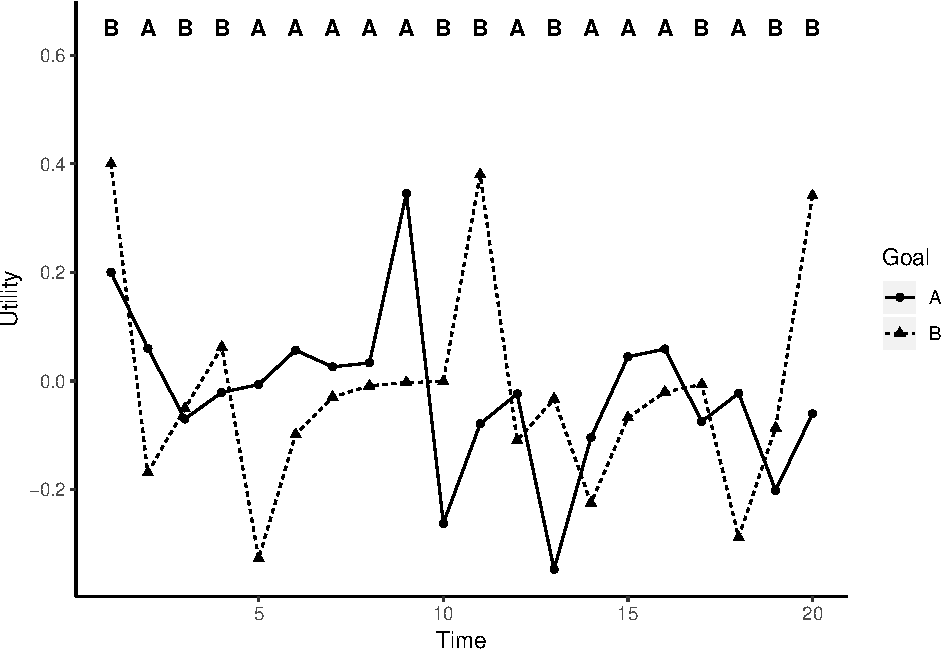
\includegraphics{figures/Figure1-1.pdf}
\caption{\label{fig:Figure1}Utility for goals \textbf{A} and \textbf{B} over
time. The letters at the top of the chart indicate which goal she chose
at each time.}
\end{figure}

\begin{figure}
\centering
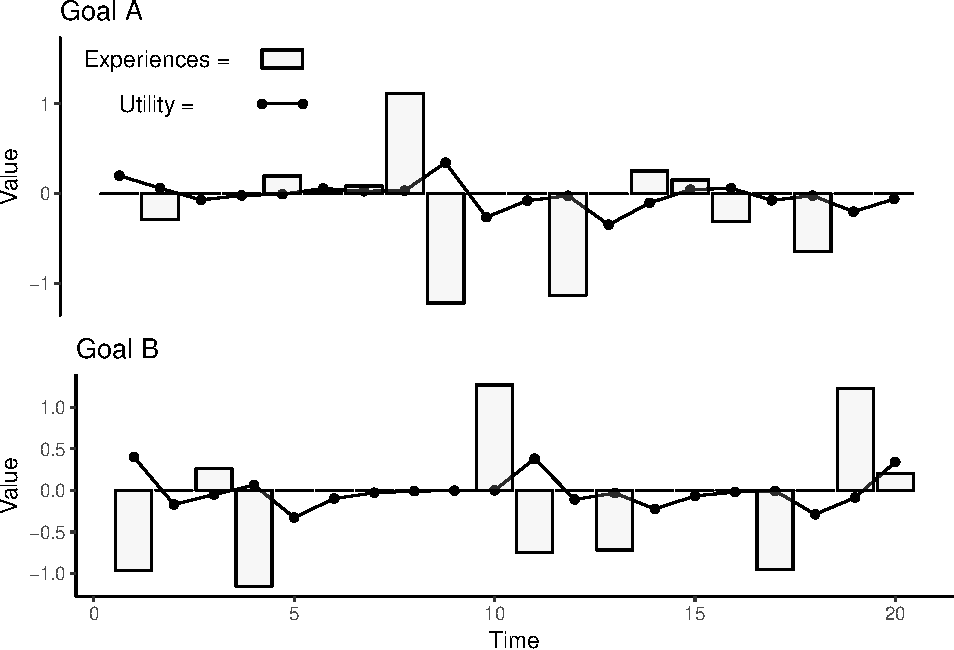
\includegraphics{figures/Figure2-1.pdf}
\caption{\label{fig:Figure2}The effect of experiences on utility across
time.}
\end{figure}

\newpage

\hypertarget{references}{%
\section{References}\label{references}}

\setlength{\parindent}{-0.5in}
\setlength{\leftskip}{0.5in}

\hypertarget{refs}{}
\leavevmode\hypertarget{ref-ackerman1996}{}%
Ackerman, P. L. (1996). A theory of adult intellectual development:
Process, personality, interests, and knowledge. \emph{Intelligence},
\emph{22}(2), 227--257.

\leavevmode\hypertarget{ref-austin1996}{}%
Austin, J. T., \& Vancouver, J. B. (1996). Goal constructs in
psychology: Structure, process, and content. \emph{Psychological
Bulletin}, \emph{120}(3), 338.

\leavevmode\hypertarget{ref-bandura2001}{}%
Bandura, A. (2001). Social cognitive theory: An agentic perspective.
\emph{Annual Review of Psychology}, \emph{52}(1), 1--26.

\leavevmode\hypertarget{ref-baumeister2016}{}%
Baumeister, R. F., Vohs, K. D., \& Oettingen, G. (2016). Pragmatic
prospection: How and why people think about the future. \emph{Review of
General Psychology}, \emph{20}(1), 3.

\leavevmode\hypertarget{ref-brydges2011}{}%
Brydges, N. M., Leach, M., Nicol, K., Wright, R., \& Bateson, M. (2011).
Environmental enrichment induces optimistic cognitive bias in rats.
\emph{Animal Behaviour}, \emph{81}(1), 169--175.

\leavevmode\hypertarget{ref-busemeyer2018}{}%
Busemeyer, J. R. (2018). Old and new directions in strategy selection.
\emph{Journal of Behavioral Decision Making}, \emph{31}(2), 199--202.

\leavevmode\hypertarget{ref-busemeyer2002}{}%
Busemeyer, J. R., Townsend, J. T., \& Stout, J. C. (2002). Motivational
underpinnings of utility in decision making. \emph{Advances in
Consciousness Research}, \emph{44}, 197--220.

\leavevmode\hypertarget{ref-cappelli1991}{}%
Cappelli, P. (1991). The missing role of context in ob: The need for a
meso-level approach. \emph{Organizational Behavior}, \emph{13}, 55--110.

\leavevmode\hypertarget{ref-Cortina2016}{}%
Cortina, J. M. (2016). Defining and operationalizing theory.
\emph{Journal of Organizational Behavior}, \emph{37}(8), 1142--1149.

\leavevmode\hypertarget{ref-Cortina2017}{}%
Cortina, J. M., Aguinis, H., \& DeShon, R. P. (2017). Twilight of dawn
or of evening? A century of research methods in the journal of applied
psychology. \emph{Journal of Applied Psychology}, \emph{102}(3), 274.

\leavevmode\hypertarget{ref-crowe1997}{}%
Crowe, E., \& Higgins, E. T. (1997). Regulatory focus and strategic
inclinations: Promotion and prevention in decision-making.
\emph{Organizational Behavior and Human Decision Processes},
\emph{69}(2), 117--132.

\leavevmode\hypertarget{ref-denissen2011}{}%
Denissen, J. J., Aken, M. A. van, \& Roberts, B. W. (2011). Personality
development across the life span. \emph{The Wiley-Blackwell Handbook of
Individual Differences}, 75--100.

\leavevmode\hypertarget{ref-denrell2005}{}%
Denrell, J. (2005). Why most people disapprove of me: Experience
sampling in impression formation. \emph{Psychological Review},
\emph{112}(4), 951.

\leavevmode\hypertarget{ref-denrell2007adaptive}{}%
Denrell, J. (2007). Adaptive learning and risk taking.
\emph{Psychological Review}, \emph{114}(1), 177.

\leavevmode\hypertarget{ref-DeShon2012}{}%
DeShon, R. P. (2012). Multivariate dynamics in organizational science.
In S. W. J. Kozlowski (Ed.), \emph{The oxford handbook of organizational
psychology} (pp. 117--142). Oxford University Press.

\leavevmode\hypertarget{ref-deshon2009}{}%
DeShon, R. P., \& Rench, T. A. (2009). Clarifying the notion of
self-regulation in organizational behavior. \emph{International Review
of Industrial and Organizational Psychology}, \emph{24}, 217--248.

\leavevmode\hypertarget{ref-dickinson1989}{}%
Dickinson, A. M. (1989). The detrimental effects of extrinsic
reinforcement on ``intrinsic motivation''. \emph{The Behavior Analyst},
\emph{12}(1), 1--15.

\leavevmode\hypertarget{ref-douglas2012}{}%
Douglas, C., Bateson, M., Walsh, C., Bédué, A., \& Edwards, S. A.
(2012). Environmental enrichment induces optimistic cognitive biases in
pigs. \emph{Applied Animal Behaviour Science}, \emph{139}(1), 65--73.

\leavevmode\hypertarget{ref-dreher1991}{}%
Dreher, G. F., \& Bretz, R. D. (1991). Cognitive ability and career
attainment: Moderating effects of early career success. \emph{Journal of
Applied Psychology}, \emph{76}(3), 392.

\leavevmode\hypertarget{ref-duman2009}{}%
Duman, R. S. (2009). Neuronal damage and protection in the
pathophysiology and treatment of psychiatric illness: Stress and
depression. \emph{Dialogues in Clinical Neuroscience}, \emph{11}(3),
239.

\leavevmode\hypertarget{ref-erez2002}{}%
Erez, A., \& Isen, A. M. (2002). The influence of positive affect on the
components of expectancy motivation. \emph{Journal of Applied
Psychology}, \emph{87}(6), 1055.

\leavevmode\hypertarget{ref-gigerenzer1999}{}%
Gigerenzer, G., Todd, P. M., \& ABC Research Group, the. (1999).
\emph{Simple heuristics that make us smart}. Oxford University Press.

\leavevmode\hypertarget{ref-grandey2000}{}%
Grandey, A. A. (2000). Emotional regulation in the workplace: A new way
to conceptualize emotional labor. \emph{Journal of Occupational Health
Psychology}, \emph{5}(1), 95.

\leavevmode\hypertarget{ref-grandey2015}{}%
Grandey, A. A., \& Gabriel, A. S. (2015). Emotional labor at a
crossroads: Where do we go from here? \emph{Annu. Rev. Organ. Psychol.
Organ. Behav.}, \emph{2}, 323--349.

\leavevmode\hypertarget{ref-greeno1994}{}%
Greeno, J. G. (1994). Gibson's affordances. \emph{Psychological Review},
\emph{101}(2), 336--342.

\leavevmode\hypertarget{ref-guadagni1983}{}%
Guadagni, P. M., \& Little, J. D. (1983). A logit model of brand choice
calibrated on scanner data. \emph{Marketing Science}, \emph{2}(3),
203--238.

\leavevmode\hypertarget{ref-hackman1976}{}%
Hackman, J. R., \& Oldham, G. R. (1976). Motivation through the design
of work: Test of a theory. \emph{Organizational Behavior and Human
Performance}, \emph{16}(2), 250--279.

\leavevmode\hypertarget{ref-Ilgen2000}{}%
Ilgen, D. R., \& Hulin, C. L. (2000). \emph{Computational modeling of
behavior in organizations: The third scientific discipline.} American
Psychological Association.

\leavevmode\hypertarget{ref-johns2006}{}%
Johns, G. (2006). The essential impact of context on organizational
behavior. \emph{Academy of Management Review}, \emph{31}(2), 386--408.

\leavevmode\hypertarget{ref-johns2010}{}%
Johns, G. (2010). Some unintended consequences of job design.
\emph{Journal of Organizational Behavior}, \emph{31}(2), 361--369.

\leavevmode\hypertarget{ref-johns2017}{}%
Johns, G. (2018). Advances in the treatment of context in organizational
research. \emph{Annual Review of Organizational Psychology and
Organizational Behavior}, \emph{5}(1), 21--46.
doi:\href{https://doi.org/10.1146/annurev-orgpsych-032117-104406}{10.1146/annurev-orgpsych-032117-104406}

\leavevmode\hypertarget{ref-johnson2011}{}%
Johnson, D. D., \& Fowler, J. H. (2011). The evolution of
overconfidence. \emph{Nature}, \emph{477}(7364), 317.

\leavevmode\hypertarget{ref-kanfer2016}{}%
Kanfer, R., \& Chen, G. (2016). Motivation in organizational behavior:
History, advances and prospects. \emph{Organizational Behavior and Human
Decision Processes}, \emph{136}, 6--19.

\leavevmode\hypertarget{ref-keeney1976}{}%
Keeney, R. L., \& Raiffa, H. (1976). \emph{Decision analysis with
multiple objectives: Preference and value tradeoffs}. Wiley\& Sons, New
York.

\leavevmode\hypertarget{ref-kerr1975}{}%
Kerr, S. (1975). On the folly of rewarding a, while hoping for b.
\emph{Academy of Management Journal}, \emph{18}(4), 769--783.

\leavevmode\hypertarget{ref-kondrashov2016}{}%
Kondrashov, D. A. (2016). \emph{Quantifying life: A symbiosis of
computation, mathematics, and biology}. University of Chicago Press.

\leavevmode\hypertarget{ref-kraiger1993}{}%
Kraiger, K., Ford, J. K., \& Salas, E. (1993). Application of cognitive,
skill-based, and affective theories of learning outcomes to new methods
of training evaluation. \emph{Journal of Applied Psychology},
\emph{78}(2), 311.

\leavevmode\hypertarget{ref-lewin1944}{}%
Lewin, K., Dembo, T., Festinger, L., \& Sears, P. (1944). Level of
aspiration. In J. Hunt (Ed.), \emph{Personality and the behavior
disorders} (pp. 333--378). Ronald Press.

\leavevmode\hypertarget{ref-luce1959}{}%
Luce, R. D. (1959). \emph{Individual choice behavior: A theoretical
analysis}. New York: Wiley.

\leavevmode\hypertarget{ref-luce1995}{}%
Luce, R. D. (1995). Four tensions concerning mathematical modeling in
psychology. \emph{Annual Review of Psychology}, \emph{46}(1), 1--27.

\leavevmode\hypertarget{ref-luce1999}{}%
Luce, R. D. (1999). Where is mathematical modeling in psychology headed?
\emph{Theory \& Psychology}, \emph{9}(6), 723--737.

\leavevmode\hypertarget{ref-ludvig2011}{}%
Ludvig, E. A., Bellemare, M. G., \& Pearson, K. G. (2011). A primer on
reinforcement learning in the brain: Psychological, computational, and
neural perspectives. In \emph{Computational neuroscience for advancing
artificial intelligence: Models, methods and applications} (pp.
111--144). IGI Global.

\leavevmode\hypertarget{ref-matheson2008}{}%
Matheson, S. M., Asher, L., \& Bateson, M. (2008). Larger, enriched
cages are associated with `optimistic'response biases in captive
european starlings (sturnus vulgaris). \emph{Applied Animal Behaviour
Science}, \emph{109}(2), 374--383.

\leavevmode\hypertarget{ref-mathieu2015}{}%
Mathieu, J. E., Kukenberger, M. R., D'innocenzo, L., \& Reilly, G.
(2015). Modeling reciprocal team cohesion--performance relationships, as
impacted by shared leadership and members' competence. \emph{Journal of
Applied Psychology}, \emph{100}(3), 713.

\leavevmode\hypertarget{ref-mcphee1981}{}%
McPhee, R. D., \& Scott Poole, M. (1981). Mathematical modeling in
communication research: An overview. \emph{Annals of the International
Communication Association}, \emph{5}(1), 159--191.

\leavevmode\hypertarget{ref-meehl1967}{}%
Meehl, P. E. (1967). Theory-testing in psychology and physics: A
methodological paradox. \emph{Philosophy of Science}, \emph{34}(2),
103--115.

\leavevmode\hypertarget{ref-meehl1978}{}%
Meehl, P. E. (1978). Theoretical risks and tabular asterisks: Sir karl,
sir ronald, and the slow progress of soft psychology. \emph{Journal of
Consulting and Clinical Psychology}, \emph{46}(4), 806.

\leavevmode\hypertarget{ref-miller2009}{}%
Miller, J. H., \& Page, S. E. (2009). \emph{Complex adaptive systems: An
introduction to computational models of social life}. Princeton
university press.

\leavevmode\hypertarget{ref-miner1980}{}%
Miner, J. B. (1980). \emph{Theories of organizational behavior}. Dryden
Press.

\leavevmode\hypertarget{ref-mitchell2009}{}%
Mitchell, M. (2009). \emph{Complexity: A guided tour}. Oxford University
Press.

\leavevmode\hypertarget{ref-monge1990}{}%
Monge, P. R. (1990). Theoretical and analytical issues in studying
organizational processes. \emph{Organization Science}, \emph{1}(4),
406--430.

\leavevmode\hypertarget{ref-morgan2015}{}%
Morgan, S. L., \& Winship, C. (2015). \emph{Counterfactuals and causal
inference}. Cambridge University Press.

\leavevmode\hypertarget{ref-morgeson2015}{}%
Morgeson, F. P., Mitchell, T. R., \& Liu, D. (2015). Event system
theory: An event-oriented approach to the organizational sciences.
\emph{Academy of Management Review}, \emph{40}(4), 515--537.

\leavevmode\hypertarget{ref-newell1973}{}%
Newell, A. (1973). You can't play 20 questions with nature and win. In
W. G. Chase (Ed.), \emph{Visual information processing}. Academic Press.

\leavevmode\hypertarget{ref-novemsky2005}{}%
Novemsky, N., \& Dhar, R. (2005). Goal fulfillment and goal targets in
sequential choice. \emph{Journal of Consumer Research}, \emph{32}(3),
396--404.

\leavevmode\hypertarget{ref-Pearl2009}{}%
Pearl, J. (2009). Causal inference in statistics: An overview.
\emph{Statistics Surveys}, \emph{3}, 96--146.

\leavevmode\hypertarget{ref-piening2013}{}%
Piening, E. P., Baluch, A. M., \& Salge, T. O. (2013). The relationship
between employees' perceptions of human resource systems and
organizational performance: Examining mediating mechanisms and temporal
dynamics. \emph{Journal of Applied Psychology}, \emph{98}(6), 926.

\leavevmode\hypertarget{ref-pinsker1970}{}%
Pinsker, H., Kupfermann, I., Castellucci, V., \& Kandel, E. (1970).
Habituation and dishabituation of the gm-withdrawal reflex in aplysia.
\emph{Science}, \emph{167}(3926), 1740--1742.

\leavevmode\hypertarget{ref-Pitariu2010}{}%
Pitariu, A. H., \& Ployhart, R. E. (2010). Explaining change: Theorizing
and testing dynamic mediated longitudinal relationships. \emph{Journal
of Management}, \emph{36}(2), 405--429.

\leavevmode\hypertarget{ref-Ployhart2010}{}%
Ployhart, R. E., \& Vandenberg, R. J. (2010). Longitudinal research: The
theory, design, and analysis of change. \emph{Journal of Management},
\emph{36}(1), 94--120.

\leavevmode\hypertarget{ref-reeve2015}{}%
Reeve, C. L., Scherbaum, C., \& Goldstein, H. (2015). Manifestations of
intelligence: Expanding the measurement space to reconsider specific
cognitive abilities. \emph{Human Resource Management Review},
\emph{25}(1), 28--37.

\leavevmode\hypertarget{ref-rescorla1972}{}%
Rescorla, R. A., \& Wagner, A. R. (1972). A theory of pavlovian
conditioning: Variations in the effectiveness of reinforcement and
nonreinforcement. \emph{Classical Conditioning II: Current Research and
Theory}, \emph{2}, 64--99.

\leavevmode\hypertarget{ref-salmeto2011}{}%
Salmeto, A. L., Hymel, K. A., Carpenter, E. C., Brilot, B. O., Bateson,
M., \& Sufka, K. J. (2011). Cognitive bias in the chick
anxiety--depression model. \emph{Brain Research}, \emph{1373}, 124--130.

\leavevmode\hypertarget{ref-schmidt2007}{}%
Schmidt, A. M., \& DeShon, R. P. (2007). What to do? The effects of
discrepancies, incentives, and time on dynamic goal prioritization.
\emph{Journal of Applied Psychology}, \emph{92}(4), 928.

\leavevmode\hypertarget{ref-shan2005}{}%
Shan, J. (2005). Does financial development `lead'economic growth? A
vector auto-regression appraisal. \emph{Applied Economics},
\emph{37}(12), 1353--1367.

\leavevmode\hypertarget{ref-shantz2009}{}%
Shantz, A., \& Latham, G. P. (2009). An exploratory field experiment of
the effect of subconscious and conscious goals on employee performance.
\emph{Organizational Behavior and Human Decision Processes},
\emph{109}(1), 9--17.

\leavevmode\hypertarget{ref-simon1956}{}%
Simon, H. A. (1956). Rational choice and the structure of the
environment. \emph{Psychological Review}, \emph{63}(2), 129.

\leavevmode\hypertarget{ref-simon1992}{}%
Simon, H. A. (1992). What is an ``explanation'' of behavior?
\emph{Psychological Science}, \emph{3}(3), 150--161.

\leavevmode\hypertarget{ref-steel2006}{}%
Steel, P., \& König, C. J. (2006). Integrating theories of motivation.
\emph{Academy of Management Review}, \emph{31}(4), 889--913.

\leavevmode\hypertarget{ref-stewart2012}{}%
Stewart, I. (2012). \emph{In pursuit of the unknown: 17 equations that
changed the world}. Basic Books.

\leavevmode\hypertarget{ref-taylor2014}{}%
Taylor, S. G., Bedeian, A. G., Cole, M. S., \& Zhang, Z. (2014).
Developing and testing a dynamic model of workplace incivility change.
\emph{Journal of Management}, \emph{43}(3), 645--670.

\leavevmode\hypertarget{ref-tett2003}{}%
Tett, R. P., \& Burnett, D. D. (2003). A personality trait-based
interactionist model of job performance. \emph{Journal of Applied
Psychology}, \emph{88}(3), 500.

\leavevmode\hypertarget{ref-thaler1990}{}%
Thaler, R. H., \& Johnson, E. J. (1990). Gambling with the house money
and trying to break even: The effects of prior outcomes on risky choice.
\emph{Management Science}, \emph{36}(6), 643--660.

\leavevmode\hypertarget{ref-thibaut1959}{}%
Thibaut, J. W., \& Kelley, H. H. (1959). \emph{The social psychology of
groups}. Routledge.

\leavevmode\hypertarget{ref-tobin2010}{}%
Tobin, R. M., \& Graziano, W. G. (2010). Delay of gratification.
\emph{Handbook of Personality and Self-Regulation}, 47--63.

\leavevmode\hypertarget{ref-vancouver2018}{}%
Vancouver, J. B., Wang, M., \& Li, X. (2018). Translating informal
theories into formal theories: The case of the dynamic computational
model of the integrated model of work motivation. \emph{Organizational
Research Methods}, 1094428118780308.

\leavevmode\hypertarget{ref-vancouver2012}{}%
Vancouver, J. B., \& Weinhardt, J. M. (2012). Modeling the mind and the
milieu: Computational modeling for micro-level organizational
researchers. \emph{Organizational Research Methods}, \emph{15}(4),
602--623.

\leavevmode\hypertarget{ref-vancouver2010}{}%
Vancouver, J. B., Weinhardt, J. M., \& Schmidt, A. M. (2010). A formal,
computational theory of multiple-goal pursuit: Integrating goal-choice
and goal-striving processes. \emph{Journal of Applied Psychology},
\emph{95}(6), 985.

\leavevmode\hypertarget{ref-van1996}{}%
Van Eerde, W., \& Thierry, H. (1996a). Vroom's expectancy models and
work-related criteria: A meta-analysis. \emph{Journal of Applied
Psychology}, \emph{81}(5), 575.

\leavevmode\hypertarget{ref-vaneerde1996}{}%
Van Eerde, W., \& Thierry, H. (1996b). Vroom's expectancy models and
work-related criteria: A meta-analysis. \emph{Journal of Applied
Psychology}, \emph{81}(5), 575.

\leavevmode\hypertarget{ref-voelkle2015relating}{}%
Voelkle, M. C., \& Oud, J. H. (2015). Relating latent change score and
continuous time models. \emph{Structural Equation Modeling: A
Multidisciplinary Journal}, \emph{22}(3), 366--381.

\leavevmode\hypertarget{ref-von1982}{}%
Von Winterfeldt, D., \& Edwards, W. (1982). Costs and payoffs in
perceptual research. \emph{Psychological Bulletin}, \emph{91}(3), 609.

\leavevmode\hypertarget{ref-worthy2007}{}%
Worthy, D. A., Maddox, W. T., \& Markman, A. B. (2007). Regulatory fit
effects in a choice task. \emph{Psychonomic Bulletin \& Review},
\emph{14}(6), 1125--1132.

\leavevmode\hypertarget{ref-yechiam2005}{}%
Yechiam, E., \& Busemeyer, J. R. (2005). Comparison of basic assumptions
embedded in learning models for experience-based decision making.
\emph{Psychonomic Bulletin \& Review}, \emph{12}(3), 387--402.


\end{document}
